\documentclass[a4paper,11pt]{article}
\usepackage[pdftex]{color}
\usepackage[pdftex]{graphicx}


\title{JABA for Haiku, BeOS and ZETA \\ {\large Just Another Burning Application} \\ \vspace{2cm} User Manual\\ \vspace{10cm}\ }
\author{DasJott, jan\_\_64}

\begin{document}

\sloppy
\newcommand{\mybaselinestretch}{0.9}
\renewcommand{\baselinestretch}{\mybaselinestretch} 

\maketitle

\thispagestyle{empty}
\newpage

\tableofcontents
\newpage


\section{Introduction to JABA}

Welcome to JABA, your all-in-one CD and DVD burning tool. It is also great at creating image files,
mastering audio CDs and copying your discs. JABA is the short form for the bulky name ``Just Another Burning Application''. Technically it is a practical user interface to a range of
complex commandline utilities -- mainly cdrecord, a fine CD and DVD recording utility 
by J\"org Schilling. (JABA will give you a complete list of used tools in it's About window.)

JABA was developed by DasJott in 2005 using the free BASIC programming language yab. Yab was specially designed for Haiku, BeOS and ZETA and JABA was the first major application written with it. First, JABA was released for ZETA exclusively. However, after the decline of ZETA the original author who still keeps the rights on the sourcecode, lost interest in JABA and the Be community.

Team Maui\footnote{\tt http://www.team-maui.org}, a group of enthusiastic developers and designers gained the rights to release JABA under the terms and conditions of the free Haiku License. The team cleaned up the code and also this manual, and replaced all images for a better Haiku style.

\subsection{Getting Started with JABA}

Starting JABA for the first time, will open a small setup window first, expecting a few
important settings from you to make. Please refer to Section 2 for more details on the
possible configuration options.

In the first window of the setup klick on "Start setup" and you'll see two checkboxes to
be checked.
The first checkbox leads you to the ``Burner Device'' settings window. Please select your
CD or DVD burner here, to let JABA know which one of your drives is now your default burner.

\begin{center}
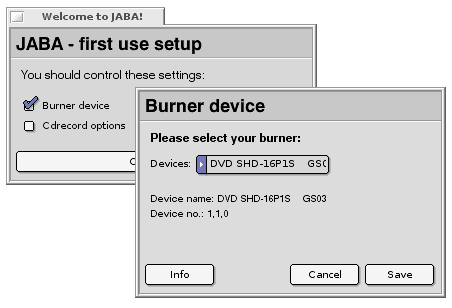
\includegraphics[width=226bp]{startsetup1.png} \\
Selecting a CD or DVD burner from the list
\end{center}

The second checkbox leads you to the ``Cdrecord Options'' settings window. Here you
can set some special options for your buner. 

\begin{center}
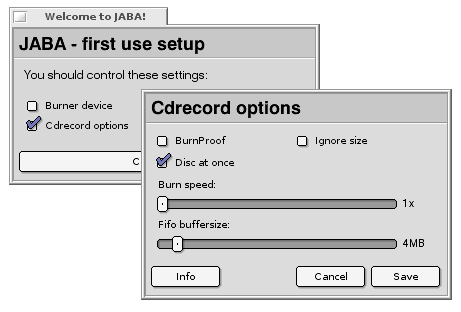
\includegraphics[width=230bp]{startsetup2.png} \\
Configuring your burner
\end{center}

\begin{center} \colorbox[gray]{.9}{ \parbox{12cm}{
Hint: If you set the speed higher than your drive is able to work with, cdrecord will set the speed as high as your drive is able to -- automatically.
}}\end{center}

You don't have to do these steps (you can press ``Quit setup'' to start JABA
immediately), but it is highly recommended to do so, to get JABA running best.

\subsection{The Default Interface}

After setup the main window of JABA appears.
You see a range of Icons, some infoviews and a listbox.. See the graphic for description:

\subsection{Selecting a Mode}

\section{Settings}

In the main-menu you can find the point "Settings", which JABA provides all important
settings with.

\subsection{Burner}

In this window JABA lists all the drives cdrecord could find. Please select your burner
device with the dropbox.
If you are not sure, which one is your burner, press the "Info"-button to get some more
information about the chosen drive.
If that also doesn't help you, please see the manual of your computer or contact the
manufactor to find out the burner device.
The "Cancel"-button will close the window without saving - the "Save"-button will save
the currently chosen drive as the burner device and then close the window.

\subsection{Cdrecord options}

Here you can find a few special options for cdrecord to set.
If your burner device supports "BurnProof", it is highly recommended to select that
point.
If the option "Size > 700MB" is set, JABA will let you burn more than the disc is able
to. Use on your own risk!
The checkbox named "Force blanking RW" lets JABA ignore errormessages that might
come up while blanking a RW-disc and simply continues blanking-process (if possible).
Set the burn speed of your burner device. You can get that info from the manual of your
burner. Usually there should be no risk to set the burn speed higher than your burner is
able to, because if it is set too high, cdrecord will use the highest speed that is possible.
For setting Fifo buffersize, please see also the manual of your burner device.
The "Info"-buttons leads you to a window containing a few infos about your currently
used cdrecord-version.
The "Cancel"-buttons closes the window without saving anything.
The "Save"-button saves the settings you made and then closes the window.

\subsection{Data Filesystem}

Here you can set the filesystem you want to use while burning data-discs.
The default is set to "Windows joliet", as the filenames are looking best on the CD after
burning.
The ISO-standard requires to fit the filenames to a standard set of characters.
Please see the tooltips for getting a bit more info about each filesystem.

\subsection{Interface}

Here you can choose between the "Standard GUI" and the "Simple GUI". GUI means
Graphical User Interface.
You are also able to change the main color of JABA. A preview of the currently set
color is given via the background of the interface-settings-window.
With the "Standard"-button, JABA's GUI is set to the standard interface and color.
The changes will appear, when you press the "Save"-button and restart JABA (close
start JABA again).
Just try it.

\section{Burn a Disk}

You set your burner device and the cdrecord options and just want to burn some files to
a disc now? Ok, then let's go.

\subsection{Burn audio-disc}

First select "Audio-disc" from the iconbar (standard GUI) or via the dropbox (simple
GUI).
Now drop some audio-files into the list. Be sure to only drop audio-files and to drop
them from a BFS-volume (e.g. the ZETA-partition).
As an audio-disc can only contain files in a special-defined format (WAV) for being
played in a HiFi-CDplayer, JABA converts every dropped file to that format - if needed.
So it may take a short time for converting, if non-WAV files were dropped, but you can
then be sure to get a real high-quality audio-disc.
You can give the project a name - though it will not be used on the disc itself (because
of the audio-cd standard) it is used, if you save the project (see 6. Project management).
The copy protection provided here may be recognized by HiFi-CDburners. If so, the
audio-disc created by JABA can not be copied.
When you completed the collection and want to burn it, press the "Burn"-button. A burn
window will be opened.
Just to be sure, the project name and the burner device name is showed in the first two
lines. Below them a few checkboxes are provided.
If you don't know the meaning of the options, just leave them on default settings (and
see "3.2 Burn data-disc").
If the "Burn!"-button is pressed, the disc will be burned - without any way back. You
can't cancel the burning-process, once started.

\subsection{Burn data-disc}

First select "Data-disc" from the iconbar (standard GUI) or via the dropbox (simple
GUI).
You can choose between burning a CD or a DVD. Corresponding to that choice, the
disc-size will be shown in the statusbar.
Now drop some files or folders into the list. You should also give that project a name, as
it will be the name of the disc, when it is burnt.
For the options "Multisession" and "Boot image" see "5. Advanced functions" in
manual.
When you completed the collection and want to burn it, press the "Burn"-button. A burn
window will be opened.
Just to be sure, the project name and the burner device name is showed in the first two
lines. Below them a few checkboxes are provided.
Streaming:
Write the files directly to the disc, without creating an imagefile first.
This means a higher risk, as an imagefile is created directly to the disc - on the fly.
In most cases that option works without problems and means less time for burning.
Fixate:
Also called "Finalise". Means that the disc will be written with a TOC (table of
contents), so that no more files can be burnt on that disc (this is not multisession!).
Without setting that option you can burn one session in a few steps - but the disk may
not be readable until it is fixated!
Disc at once:
Opposite to "Track at once". Means that all data is written as one track on the CD.
Eject disc when finished:
Ejects the disc after burning it.
Keep image and save as:
When you set that option, a filepanel will open expecting a name to save the created
imagefile with.
If streaming is set this option is disabled, as streaming means no creation of an imagefile
on the harddisk.
Quit when finished:
Quits JABA after burning the disc.

\subsection{Copy disc}

Select "Copy disc" from the "Disc"-menu or from the iconbar in standard GUI.
A copy-window opens then, providing further options.
You have to select, if you want to copy a data-disc or a audio-disc. Copying an audio-
disc while using "Copy data disc" will NOT work! Also note, that there won't be created
any imagefile when copying an audio-disc!
Because of the special way of copying audio-discs used in JABA, some options will be
disabled when set to "Copy audio disc".
Next select the source device to copy from. It is understood, that the option "On the fly"
(aka direct-copy) is disabled, if source and target device is the

\section{Imagefiles}

JABA is able to create, read and burn imagefiles. You can also use CUE-files with
JABA.
Take a look in the "Image"-menu or (for standard GUI use) in the iconbar below the
menu.

\subsection{Create imagefile}

For creating an imagefile with JABA, you just have to drop some files into the list and
select "Create imagefile" from the menu or the iconbar. A filepanel opens to let you
choose the name and place to save the imagefile. After typing in the name, press the
"Save"-button to create an imagefile from the current project.

\subsection{Read image from disc}

Reading discs and creating an imagefile from it. Does only work with data-discs!
After selecting this function, a filepanel opens expecting a name and place to save the
imagefile to, once it is created. Type one in and press the "Save"-button.
After doing that, a small window opens where you can set the device which contains the
disc to read the imagefile from.

\subsection{Burn imagefile}

If this function is chosen, a filepanel opens expecting you to selct an imagefile.
Select one and press the "Open"-button to get to the next window.
In that window you can also set "Fixate". In this case, it means that the disc will not be
finished, so you can burn another imagefile on the same disc.

\subsection{Burning CUE-file}

Some imagefiles (or sets of imagefiles) may provided with a CUE-file.
A CUE-file is kind of a "manual how to burn the imagefile(s)".
So if you got imagefile(s) together with such a CUE-file, it's recommended to use it.
After selecting this function a filepanel opens expecting you to choose the CUE-file.
Select one and press the "Open"-button to get to the next window, wher you can set the
same options as in "Burn imagefile".

\section{Advanced functions}

Like the functions described under 4. wouldn't be enough, JABA provides some special
functions for burning. For details read the following.

\subsection{Multisession}

Multisession discs are disc, that can be written in more than one step. Therefore it is
written a special TOC after each session. If you think the disc is finished and want to
burn the real last session on that disc, you can also fixate it, as described below.
Creating multisession discs with JABA is really easy.
For the first session just set the "Multisession"-checkbox on active and burn the session.
For any further session simply do the same - set "Multisession" and burn the session.
JABA automatically detects, if it is the first session or if it is a further session.
When you want to finish (fixate) the disc, set the "Last session"-checkbox in the burn
window appering after pressing the "Burn"-button.

\subsection{Blank RW-disc}

To blank a RW-disc select this function. Description of the options:
Blank fast:
This option is recommended, as it is adequate in most cases.
Blank all:
This option will take much more time than the "Blank fast"-option, as the whole disc will
be blanked. So be very patient, if chosen this.
Blank last session:
Will blank the last session of a multisession-disc - if it's not fixated.

\subsection{Fixate disc}

If you have got a disc, which you think it is not fixated you can do that single step with
this function.

\section{Project management}

You collected some files/folders in JABA but want to burn it some time later?
No problem, just save your project. For that select "Save project" in the "File"-menu. A
filepanel opens expecting a name for the project.
The standard-projectfolder is always opened first in this filepanel. It is recommended to
save all projects in that directory, as you have a fast access that way.
Saving projects to other directories on your ZETA-partition is also no problem.
Note:
Please only save projectfiles on BFS-volumes! Otherwise you won't be able to load them
back to JABA.
For each project a projectfile and a folder will be created. The folder contains the
folder-structure and the files as links. The projectfile itself is the one to be loaded, to get
the project back to
JABA will only load projectfiles created with JABA.

\section{Frequently Asked Questions}

What is JABA?

      JABA is a graphical user interface. It uses commandline-tools for doing the work,
      especially cdrecord to burn discs.

How do I get the files and folders I'd like to burn into JABA?

      As usual in ZETA drag'n'drop is used for JABA. That means, that you can simply
      drag the files and folders from Tracker and drop them onto the listfield.

Does JABA not provide fullscreen-view?

      As files and folders can only be added via drag'n'drop from Tracker, it is important
      that there is enough place left, when pressed the zoom-button in the tab.

Sometimes JABA takes a few seconds while adding data to the list?

      JABA takes care of your data. It uses a temporary system, so your data is save
while
      removing, moving, adding and browsing in JABA.
      Audiofiles are always converted to the required format, so you should
      always get best results for audio-discs.

I can't drop my audiofiles for creating an audio-disc?

      Copy the files to a BFS-volume like your ZETA-partition. Then select them all
and
      rightclick them. Choose "Indentify" in the Tracker-menu.
      JABA needs the file-attributes used on BFS to recognize audio-data.

The displayed playtime in JABA in audiomode isn't correct?

      Yes, sometimes it happens, that compressed wav-data causes the time-display to

\end{document}
